%% example-1.Rnw

\documentclass[a4paper]{article}

\title{Sweave Example 1}
\author{Friedrich Leisch}

\usepackage{Sweave}
\usepackage[12hr]{datetime}
\usepackage{datenumber} 

%%https://tex.stackexchange.com/questions/167751/latex-usepackagedatetime-and-usepackagescrtime-are-off-by-an-hour

%% Define timezone
\usepackage{etoolbox}


\def\parsepdfdatetime#1:#2#3#4#5#6#7#8#9{%
	\def\theyear{#2#3#4#5}%
	\def\themonth{#6#7}%
	\def\theday{#8#9}%
	\parsepdftime
}

\def\parsepdftime#1#2#3#4#5#6#7\endparsepdfdatetime{%
	\def\thehour{#1#2}%
	\def\theminute{#3#4}%
	\def\thesecond{#5#6}%
	\ifstrequal{#7}{Z}
	{%
		\def\thetimezonehour{+00}%
		\def\thetimezoneminute{00}%
	}%
	{%
		\parsepdftimezone#7%
	}%
}

\def\parsepdftimezone#1'#2'{%
	\def\thetimezonehour{#1}%
	\def\thetimezoneminute{#2}%
}

\newcommand*{\thetimezone}{\thetimezonehour:\thetimezoneminute}

\begin {document}


\expandafter\parsepdfdatetime\pdfcreationdate\endparsepdfdatetime

\newdateformat{mydate}{\datedayname, \monthname[\the\month] \the\day 
\textsuperscript{th},  
\the\year, 
\currenttime \hspace{0.25em} [Time Zone GMT \thetimezone]}

\mydate
\maketitle 

In this example we embed parts of the examples from the
\texttt {kruskal.test} help page into a \LaTeX{} document :


\begin{Schunk}
\begin{Sinput}
> data(airquality,package="datasets")
> library("stats")
> kruskal.test(Ozone ~ Month,data = airquality)
\end{Sinput}
\begin{Soutput}
	Kruskal-Wallis rank sum test

data:  Ozone by Month
Kruskal-Wallis chi-squared = 29.267, df = 4, p-value = 6.901e-06
\end{Soutput}
\end{Schunk}

which shows that the location parameter of the Ozone
distribution varies significantly from month to month. Finally , we
include a boxplot of the data , using
%% want an eval = FALSE case and referencing a previous chunk :

\begin{Schunk}
\begin{Sinput}
>   boxplot(Ozone ~ Month,data = airquality)
\end{Sinput}
\end{Schunk}
  
\begin{center}
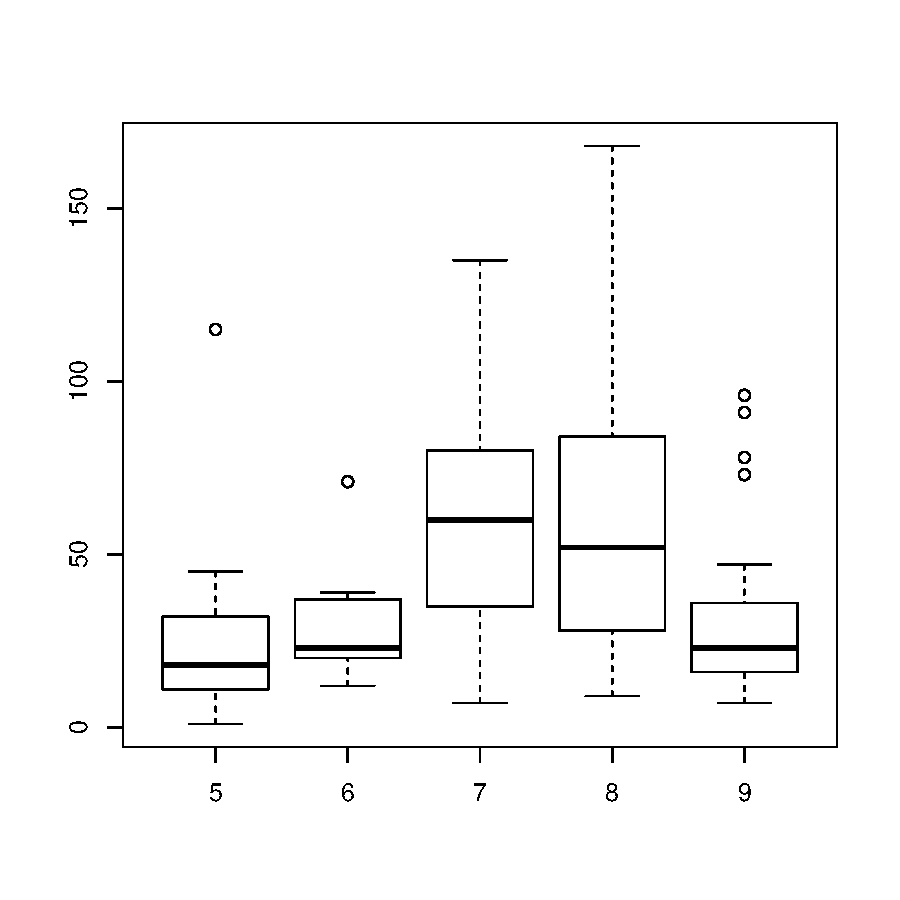
\includegraphics{example-1-003}
\end{center}


\end{document}
